\chapter{Background}
\label{cha:background}

In this thesis, we will analyze in detail the behavior of an LLM as an agent within
a controlled environment.

Before presenting all the work carried out in detail, this chapter aims to
provide a comprehensive explanation of all the theoretical foundations necessary
to understand the steps presented in the following chapters. Starting from a brief
introduction of Artificial Intelligence just to define the boundaries in which we
are working, we will move to the core concepts. In particular, we want to
highlight what an LLM is and how it works, with a special focus on the Attention
mechanism and how the uncertainty of an LLM can be calculated. This will serve
as a basis for correctly interpreting the results analyzed in Section
\ref{cha:results_discussion}.

There will also be a broader discussion on agents in a strict sense and ``LLM
agents" to better show the difference between our implementation and what is currently
being discussed in the literature.

To better define the context of this thesis, we will also examine the main
alternative approaches to solving a logistical problem currently studied in the
literature.

\section{Artificial Intelligence}
\label{sec:artificial_intelligence}

Artificial Intelligence (AI) is a very wide field, that can be resumes as
systems designed to perform tasks traditionally intelligence, such as \emph{natural
language understanding}, visual perception, decision-making, and problem-solving.

In recent years, AI has rapidly evolved, driven by advances in deep learning\footnote{\url{https://en.wikipedia.org/wiki/Deep_learning}},
increased computational power, and the easy availability of massive datasets (models
are even trained on the entirety of the internet). Early AI systems, including
expert systems and early machine learning models, relied on manually crafted rules
or statistical techniques. However, with the rise of neural networks,
particularly deep learning models, AI has shifted toward self-learning systems capable
of extracting complex patterns from raw data.

One of the key breakthroughs in this evolution was the development of deep neural
networks (DNNs), particularly Convolutional Neural Networks (CNNs) for image
processing, introduced by Krizhevsky et al. \cite{articleCNN} and Recurrent
Neural Networks (RNNs) for sequential data, including language modeling,
introduced by Hochreiter et al. \cite{articleRNN}.

Despite their success, RNNs struggled with long-term dependencies due to
vanishing gradients\footnote{\url{https://en.wikipedia.org/wiki/Vanishing_gradient_problem}},
leading to the development of the \emph{Transformer architecture} (from Vaswani
et al., Attention Is All You Need \cite{vaswani2023attentionneed}), which
eliminated recurrence in favor of self-attention mechanisms, significantly improving
efficiency and scalability in natural language processing. This shift enabled
the emergence of large-scale AI models, particularly in NLP, where two main
categories dominate: discriminative models and generative models.

\paragraph{Discriminative models}
are a class of machine learning models that aim to directly model the decision
boundary between different classes in a dataset. Unlike generative models, which
learn the underlying distribution of the data, discriminative models focus on learning
the conditional probability of a target class given the input features.
Classical models like Support Vector Machines\footnote{\url{https://en.wikipedia.org/wiki/Support_vector_machine}}
and Conditional Random Fields\footnote{\url{https://en.wikipedia.org/wiki/Conditional_random_field}}
have been widely used for text classification and sequence labeling tasks such
as Named Entity Recognition (Lafferty et al. \cite{crf}). More recently, deep learning-based
models like BERT (Devlin et al. \cite{devlin2019bertpretrainingdeepbidirectional})
have been invented, that leverage contextualized word representations to improve
performance on tasks like sentiment analysis, intent detection, and slot filling.

\paragraph{Generative models}
learn the underlying data distribution to create new samples that resemble the
original data. This category includes several architectures that have pushed the
boundaries of AI-generated content. Variational Autoencoders (Kingma and Welling
\cite{kingma2022autoencodingvariationalbayes}) introduced a probabilistic
approach to generating structured data, while Generative Adversarial Networks (Goodfellow
et al. \cite{goodfellow2014generativeadversarialnetworks}) refined the concept
by using two competing neural networks, a generator and a discriminator, to
iteratively improve synthetic data generation. More recently, diffusion models (Ho
et al. \cite{ho2020denoisingdiffusionprobabilisticmodels}) have surpassed GANs in
generating high-quality images by modeling data transformations through iterative
denoising processes. In the domain of text generation, autoregressive models like
GPT (Radford et al. \cite{radford2018improving}) demonstrated the power of large-scale,
unsupervised pretraining. These Large Language Models predict the next token (that
can be seen as a building block of a word, approximately a syllable) in a sequence
based on vast amounts of textual data, learning contextual nuances and producing
human-like responses.

\section{Large Language Models - LLMs}
\label{sec:large_language_models_llms}

Large Language Models (LLMs) are a class of deep learning models that leverage transformer
architectures to generate coherent and contextually relevant text. These models
have revolutionized natural language processing by achieving state-of-the-art
performance on a wide range of tasks, including language modeling, translation, summarization,
and question-answering.

The transformer architecture, introduced by Vaswani et al. in the paper ``Attention
Is All You Need" \cite{vaswani2023attentionneed}, is the foundation of LLMs. It consists
of an encoder-decoder structure, where the encoder processes the input sequence
and generates a sequence of hidden states, while the decoder generates the output
sequence based on the encoder's hidden states. The key innovation in
transformers is the self-attention mechanism, which allows the model to weigh the
importance of different input tokens when generating the output. This mechanism
enables transformers to capture long-range dependencies and contextual
information more effectively than RNNs.

In this thesis, we will focus on the models built by OpenAI, we will analyze
them more in depth in Section \ref{sec:llm_models}.

\begin{figure}[h!]
  \centering
  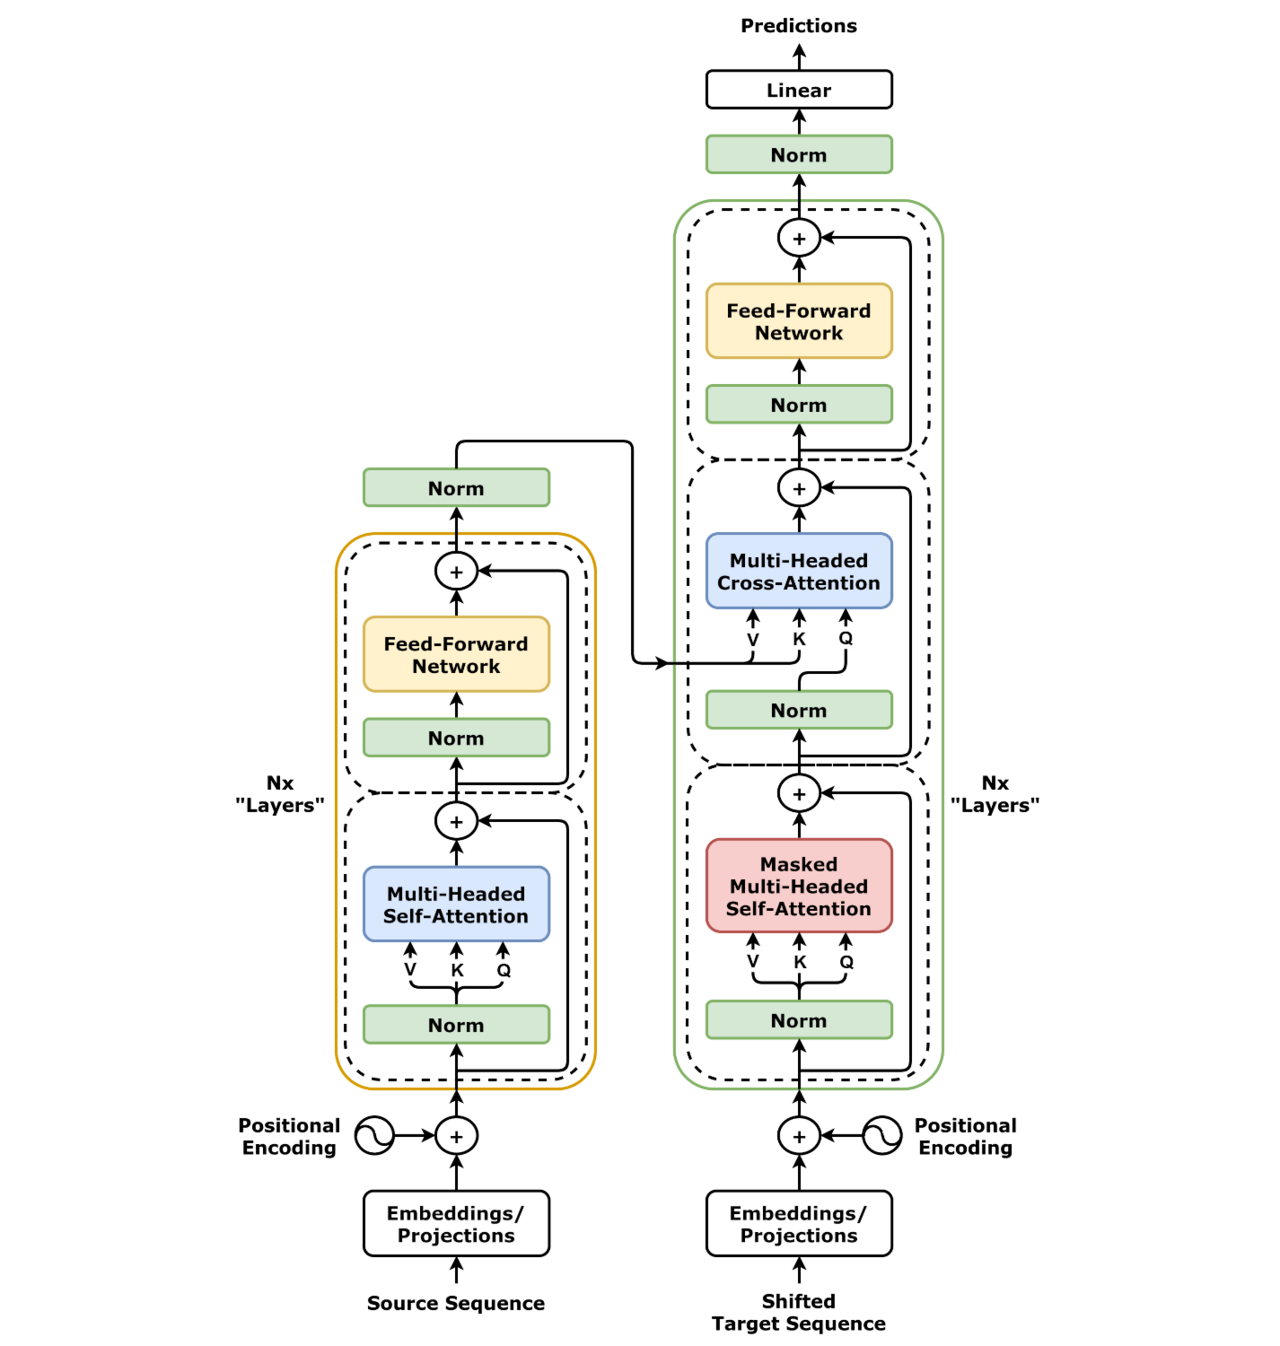
\includegraphics[width=0.65\textwidth]{images/transformer_architecture.png}
  \caption{Transformer Architecture}
  {\emph{Source: Vaswani et al., Attention Is All You Need \cite{vaswani2023attentionneed}}}
  \label{fig:transformer_architecture}
\end{figure}

\subsection{Attention Mechanism}
\label{sub:attention_mechanism}

The attention mechanism is a fundamental component of the transformer
architecture (Figure \ref{fig:transformer_architecture}), enabling the model to focus
on specific parts of the input sequence when generating the output. The
attention mechanism computes a weighted sum of the input tokens, where the weights
are learned during training based on the relevance of each token to the current context.

The self-attention mechanism works in this way:
\begin{enumerate}
  \item create 3 vectors from embeddings (query, key, value) multiplying by 3 matrices
    learned during the training process;

  \item calculate a score that determines how much focus goes to different parts
    of the input sentence as it encodes a word;

  \item divide the score for more stable gradients and apply softmax;

  \item multiply each value vector by the softmax score to keep the value of the
    word it focuses on, and sink other irrelevant words;

  \item sum the weighted value vectors: this produces the output of the self-attention
    layer at this position.
\end{enumerate}

The self-attention operation computes the relevance of each token in the input with
respect to the query token using the scaled dot-product attention:

\begin{displaymath}
  \mbox{Attention}(Q, K, V) = \mbox{softmax}\left(\frac{QK^{T}}{\sqrt{d_{k}}}\right
  ) V
\end{displaymath}

where $d_{k}$ is the dimensionality of the key vectors, ensuring that the dot products
do not grow too large as input size increases. The softmax function normalizes
the scores into attention weights, which determine how much influence each token
should have on the final representation.

Multi-head attention extends this mechanism by computing multiple sets of $Q,K,V$
matrices in parallel, allowing the model to capture different aspects of
contextual relationships:

\begin{displaymath}
  \mbox{MultiHead}(Q, K, V) = \mbox{Concat}(\mbox{head}_{1}, \dots, \mbox{head}_{h}
  ) W^{O}
\end{displaymath}

where each attention head independently applies scaled dot-product attention,
and the outputs are concatenated and linearly projected using $W^{O}$ . This
improves the model's ability to encode complex dependencies and contextual
meaning.

The attention mechanism allows the model to focus on different parts of the
input sequence based on the current context, enabling it to capture long-range dependencies
and improve performance on tasks like text generation.

\subsection{LLMs' Uncertainty}
\label{sub:llms_uncertainty}

Despite their impressive capabilities, LLMs are inherently probabilistic and can
generate responses that are syntactically correct yet factually inaccurate.
Understanding and quantifying this uncertainty is crucial for evaluating the
reliability of generated text, especially in high-stakes applications such as medical
diagnosis, legal advice, or automated decision-making.

For example, if an LLM generates an answer to a yes/no question with
probabilities:
\begin{displaymath}
  P(\mbox{Yes})=0.51,P(\mbox{No})=0.49
\end{displaymath}

then the model is nearly uncertain, and this information should be communicated rather
than presenting ``Yes" as a definitive response.

A key consequence of uncertainty is the phenomenon of \emph{hallucination},
where the model generates confident but factually incorrect or fabricated
information \cite{Ji_2023}. Hallucinations arise when:
\begin{itemize}
  \item the model lacks knowledge about a specific query but still generates an answer;

  \item the training data contains conflicting or misleading patterns;

  \item the model overgeneralizes from limited training examples.
\end{itemize}

Mitigating hallucinations involves uncertainty-aware generation techniques, the
most common one is \emph{Retrieval-Augmented Generation} (RAG) \cite{lewis2021retrievalaugmentedgenerationknowledgeintensivenlp},
which enhance the prompt with additional context from a knowledge base to
improve the model's factual accuracy.

The literature studied different approaches to quantify uncertainty in LLMs, and
this thesis will use one of the most common methods to quantify the probability of
correctness in the generated choice by the agent.

\subsubsection{Expressing Uncertainty}
A study titled ``Can LLMs Express Their Uncertainty? An Empirical Evaluation of
Confidence Elicitation in LLMs" \cite{xiong2024llmsexpressuncertaintyempirical} investigates
methods for eliciting confidence from LLMs without accessing their internal parameters
or fine-tuning. The researchers propose a framework comprising three components:
\begin{itemize}
  \item Prompting Strategies: Techniques to elicit verbalized confidence from
    the model;

  \item Sampling Methods: Generating multiple responses to assess variability;

  \item Aggregation Techniques: Computing consistency across responses to
    determine confidence levels.
\end{itemize}

The study evaluates these methods on tasks such as confidence calibration and
failure prediction across various datasets and LLMs, including GPT-4 and LLaMA 2
Chat.

Key findings indicate that LLMs often exhibit overconfidence when verbalizing their
certainty, possibly mirroring human confidence expression patterns. Additionally,
as model capabilities increase, both calibration and failure prediction performance
improve, though they remain suboptimal. They shown that implementing strategies like
human-inspired prompts and assessing consistency among multiple responses can mitigate
overconfidence. Notably, while methods requiring internal model access perform better,
the performance gap is narrow.

\subsubsection{Stable Explanations as Confidence Measures}
In the pursuit of reliable uncertainty quantification in Large Language Models, the
paper ``Cycles of Thought: Measuring LLM Confidence through Stable Explanations
'' \cite{becker2024cyclesthoughtmeasuringllm} introduced a novel framework that assesses
model confidence through the stability of generated explanations.

Their approach posits that the consistency of explanations accompanying an answer
can serve as a proxy for the model's certainty. Instead of assigning a single
probability to an answer, the method generates multiple explanations for the same
question and treats each explanation-answer pair as a distinct classifier. A
posterior distribution is then computed over these classifiers, allowing for a principled
estimation of confidence based on explanation stability. If the model's
explanations remain stable across different reasoning paths, it suggests high confidence
in the answer. Conversely, significant variation in explanations signals uncertainty.
Empirical evaluations across multiple datasets demonstrated that this framework
enhances confidence calibration and failure prediction, outperforming traditional
baselines.

However, there are some potential drawbacks. The method requires generating multiple
explanations, which increases computational cost and latency. Additionally, it
can be sensitive to prompt variations, and may misinterpret repetitive patterns as
high confidence.

\subsubsection{Tokens' log-probability}
\label{ssub:tokens_log_probability} The paper `Robots That Ask For Help: Uncertainty
Alignment for Large Language Model Planners'
\cite{ren2023robotsaskhelpuncertainty} introduces the KnowNo framework, which is
the one we took inspiration from to quantify the uncertainty of the agent in this
thesis.

The KnowNo framework leverages Conformal Prediction (CP)\footnote{\url{https://en.wikipedia.org/wiki/Conformal_prediction}},
a statistical method that provides formal guarantees on the reliability of predictions,
to assess uncertainty.

In the paper, they ask the LLM to generate a set of five action for a given prompt
(since the \texttt{logit\_bias} parametere in the OpenAI API was limited to five
tokens at that time), and then they ask again for the action to select. This
will not be the case of this thesis, since the actions will always be the same,
but we will use the same math behind the uncertainty calculation.

KnowNo computes uncertainty evaluating the ``validity" of each option. For each
action, CP calculates a confidence interval based on previous data and task context,
and from this, a set of valid actions is generated. This set can include one or
more actions, and the size of this set is indicative of the level of uncertainty:
\begin{itemize}
  \item Singleton: If CP narrows down the options to just one action, this indicates
    low uncertainty, and the robot can proceed confidently with the task. The model
    is highly certain that this action is the most appropriate next step.

  \item Multiple Options: When CP leaves multiple possible actions in the valid
    set, this may indicate high uncertainty. In such cases, KnowNo triggers the robot
    to request human assistance. This allows the robot to seek clarification
    when it is unsure, thereby avoiding errors that might arise from acting on uncertain
    predictions.
\end{itemize}

Technically speaking, the computation of the uncertainty can be summarize in 5
steps:
\begin{enumerate}
  \item give each action a single-token label (eg. \texttt{A)}, \texttt{B)}, \texttt{C)},
    \texttt{D)}, \texttt{E)});

  \item use the \texttt{logit\_bias} parameter in the API to force the model to
    only answer using these labels;

  \item get the log-probabilities of the tokens and scale them;

  \item filter the resulting set of option with a threshold computed with CP;

  \item either the result will be a singleton or a set of options.
\end{enumerate}

They also say that the framework has the advantage of being model-agnostic, as it
can be applied to LLMs out-of-the-box without requiring any fine-tuning, thanks
to the ``caution" that is given if the resulting filtered set of options is not a
singleton.

\section{Agents}
\label{sec:agents}

% \begin{figure}[h!]
%   \label{fig:agent_scheme}
%   \centering
%   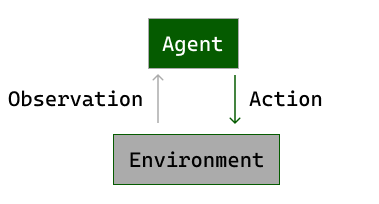
\includegraphics[width=.3333\textwidth]{images/Agent_Scheme.png}
%   \caption{Agent Scheme}
%   { Source: redesign of a scheme in \cite{wooldridge2002multiagent}}
% \end{figure}

As widely explained in the book ``An Introduction to Multiagent Systems"
\cite{wooldridge2002multiagent}, we can summarize the definition of an agent as an
autonomous entity that perceives its environment through sensors and acts upon it
through effectors, making decisions based on its perceptions and objectives in
order to achieve specific goals.

This definition highlights several key aspects of agents:
\begin{itemize}
  \item Autonomy: Agents operate without direct human intervention, controlling their
    own actions.

  \item Perception and Action: They interact with the environment via sensors (perception)
    and effectors (action execution).

  \item Decision-making: Agents select actions based on their internal model, goals,
    and the state of the environment.

  \item Non-determinism and Adaptability: Since environments are generally non-deterministic,
    agents must be prepared for uncertainty and potential failures in action execution.

  \item Preconditions and Constraints: Actions are subject to certain conditions
    that must be met for successful execution.
\end{itemize}

Thus, an agent's fundamental challenge is deciding which actions to perform in order
to best satisfy its objectives, given the constraints and uncertainties of its
environment.

\vspace{1cm} % Add margin on top
\begin{figure}[h!]
  \centering
  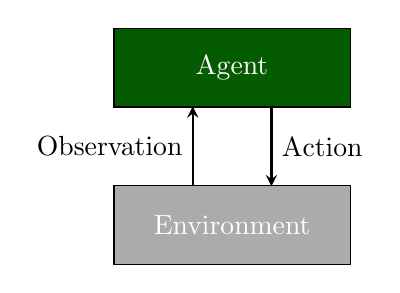
\begin{tikzpicture}[
    node distance=2cm, % Distance between nodes
  ]
    \node[
      rectangle,
      minimum width=3cm,
      minimum height=1cm,
      text centered,
      draw=black,
      fill={rgb,255:red,5; green,91; blue,0},
      text=white
    ] (agent) {Agent};
    \node[
      rectangle,
      minimum width=3cm,
      minimum height=1cm,
      text centered,
      draw=black,
      below of=agent,
      fill={rgb,255:red,171; green,171; blue,171},
      text=white
    ] (env) {Environment};

    % First arrow (Action) slightly shifted right
    \draw[thick, ->, >=stealth]
      (agent.south)
      ++(0.5,0) -- ++(0,-1)
      node[midway, right] {Action};

    % Second arrow (Observation) slightly shifted left
    \draw[thick, ->, >=stealth]
      (env.north)
      ++(-0.5,0) -- ++(0,1)
      node[midway, left] {Observation};
  \end{tikzpicture}
  \caption{Agent Design Scheme}
  {\emph{Source: redesign of a scheme in \cite{wooldridge2002multiagent}}} \label{fig:agent_scheme}
\end{figure}
\vspace{1cm} % Add margin on bottom

As shown in Figure \ref{fig:agent_scheme}, an agent is some entity that
perceives the environment and reacts to it. The setting can be anything from a simple
thermostat to a complex system like a self-driving car. The idea is that the
agent is able to react to a change in the environment and take actions to
achieve its goals.

We will analyze in detail the prompts and the choices in the Chapter
\ref{cha:data_collection} Section \ref{sec:prompts}, but to give an some anticipation
to align our agent with the definition above, we can map some of its concept to
what this thesis will analyze:
\begin{itemize}
  \item Perception and Action: what the server sends about the current state of
    the environment can be seen as the perception of the agent, while the action
    it can take will be given in the prompt in a specific way.

  \item Decision-making: the decision-making process will be the generation of
    the text by the LLM, weighted by the uncertainty.

  \item Non-determinism and Adaptability: to emulate the non-determinism of the
    environment, the state received by the server will be used ``raw" in the
    prompt, without any hard processing or parsing.

  \item Preconditions and Constraints: being in a ``limited" map with a fixed number
    of cells, is itself a constraint the agent must consider.
\end{itemize}

\subsection{BDI Architecture}
\label{sub:bdi_architecture}

The Belief-Desire-Intention (BDI) architecture is a widely adopted framework in artificial
intelligence (AI) for modeling rational agents. It was formally developed by Rao
and Georgeff in 1995 \cite{bdi-icmas95} and has been implemented in several
architectures, including PRS (1987), dMARS (1998), JAM (1999), Jack (2001), and JADEX
(2005). BDI provides a structured approach to practical reasoning, allowing agents
to function effectively in dynamic and unpredictable environments.

\subsubsection{Core Components of BDI}
BDI agents operate based on three key components:
\begin{itemize}
  \item Belief: Represents the agent's knowledge about the world, including past
    events and observations;

  \item Desire (Goals): Defines the agent's objectives or preferred end states;

  \item Intention: Represents the commitments of an agent toward achieving
    specific goals through selected plans.
\end{itemize}

BDI has been extensively used in fields like robotics, automated planning, and multi-agent
systems.

\section{State of the Art}
\label{sec:state_of_the_art}

A logistic problem is a fundamental challenge in the field of Artificial
Intelligence (AI), since depending on the complexity of the specific problem, it
can contain tasks such as route optimization, supply chain management, and
delivery scheduling. These problems arise in various domains, including
transportation, e-commerce, and manufacturing, where efficient resource allocation
and decision-making are critical. Given the complexity of modern logistics, AI has
emerged as a powerful tool for finding optimal or near-optimal solutions.

Traditional research techniques, such as linear programming and heuristics, have
been widely employed. However, with the increasing availability of data and computational
power, machine learning (ML) and deep learning methods have become more
prevalent. These methods can predict demand, optimize routes dynamically, and enhance
decision-making under uncertainty based on the data. Additionally, reinforcement
learning (RL) has gained attention for its ability to learn optimal strategies through
trial and error, particularly in dynamic and unpredictable environments.

In the recent years with the explosion of Large Language Models (LLMs), many researchers
started to apply them to different fields, including planning and logistics.

% \begin{quotation}
%   This is a longer blockquote that may span multiple paragraphs. It is indented
%   on both sides.
% \end{quotation}

\subsection{PDDL Based Solutions}
\begin{blockquote}
  \textbf{Planning Domain Definition Language} (PDDL) is a human-readable format
  for problems in automated planning that gives a description of the possible
  states of the world, a description of the set of possible actions, a specific
  initial state of the world, and a specific set of desired goals.

  \emph{Source: Wikipedia\footnotemark}
\end{blockquote}
\footnotetext{\url{https://en.wikipedia.org/wiki/Planning_Domain_Definition_Language}}

The fundamental distinction between a PDDL-based solution and any Machine
Learning/Deep Learning approach lies in the very nature of how problems are
defined and solved.

In a PDDL-based system, the problem must be explicitly encoded using a formal,
structured language that describes the initial state, the goal state, and the
set of available actions. This formal encoding serves as a blueprint for the planner,
which then performs the computationally intensive task of exploring a vast
search space. The planner systematically generates and evaluates possible action
sequences, using algorithms to determine an optimal path from the initial state
to the goal state. This process is highly deterministic, with each action being
considered in the context of its direct impact on reaching the goal.

While effective in structured, static environments with well-defined parameters,
this approach is inherently time-consuming and computationally demanding. The planner
must traverse a potentially enormous state space, guided by heuristics to prune
less relevant possibilities, but still constrained by the rigid formalism of PDDL.
Because of this, it can struggle with real-time decision-making, particularly in
situations where the environment is dynamic, uncertain, or rapidly changing.

\vspace{10mm}
\begin{codewindow}
  [PDDL Code] \lstset{style=pddlstyle, language=PDDL, caption={Domain file example for a bit toggle problem},
  label={lst:domain_file_toggle_bits}} \begin{lstlisting}
(define (domain bit-toggle)
  (:requirements :strips :negative-preconditions)
  (:predicates
    (bit ?b)                       ; predicate meaning
                                   ; bit ?b is set (true)
  )

  (:action setbit
    :parameters (?b)
    :precondition (not (bit ?b))   ; can only set a bit if
                                   ; it is not already set
    :effect (bit ?b)               ; setting the bit to true
  )

  (:action unsetbit
    :parameters (?b)
    :precondition (bit ?b)         ; can only unset a bit if
                                   ; it is currently set
    :effect (not (bit ?b))         ; setting the bit to false
  )
)

\end{lstlisting}
\end{codewindow}
\vspace{10mm}

\vspace{10mm}
\begin{codewindow}
  [PDDL Code] \lstset{style=pddlstyle, language=PDDL, caption={Problem file example for a bit toggle problem},
  label={lst:problem_file_toggle_bits}} \begin{lstlisting}
(define (problem bit-toggle-full-problem)
  (:domain bit-toggle-full)
  (:objects
     b1 b2 b3
  )
  (:init)                          ; Initially all bits are unset (false)

  (:goal                           ; It can be any combination of T/F
     (and (bit b1) (bit b2) (not(bit b3)))
  )
)
\end{lstlisting}
\end{codewindow}
\vspace{10mm}

With the increasing number of variables (actions or predicates), the number of arcs
and nodes grows exponentially. A little example that makes this problem easy to
visualize is the Domain where we can have N possible bits, that can be turned to
\texttt{true} or \texttt{false} (Domain file in Listing
\ref{lst:domain_file_toggle_bits}) and the Problem where everything start at \texttt{false}
and we want a specific final combination (Problem file in Listing \ref{lst:problem_file_toggle_bits}).

\begin{figure}[h!]
  \noindent
  \begin{minipage}{0.33\textwidth}
    \centering
    \begin{tikzpicture}[
      scale=0.8,
      transform shape,
      nodes={draw, circle, minimum size=5mm, inner sep=0pt}
    ]
      % First plot
      \node (00) at (0,0) [fill=primary, text=white] {00};
      \node (01) at (2,1) [fill=code-bg] {01};
      \node (10) at (2,-1) [fill=code-bg] {10};
      \node (11)
        at
        (4,0)
        [fill=code-bg, thick, draw=primary, line width=1mm]
        {11};
      \draw (00) -- (01);
      \draw (00) -- (10);
      \draw (01) -- (11);
      \draw (10) -- (11);
    \end{tikzpicture}

    \vspace{1cm} % Space between first and second plot

    \begin{tikzpicture}[
      scale=0.8,
      transform shape,
      nodes={draw, circle, minimum size=5mm, inner sep=0pt}
    ]
      % Second plot
      \node (000) at (0,0) [fill=primary, text=white] {000};
      \node (001) at (2,1) [fill=code-bg] {001};
      \node (010) at (2,-1) [fill=code-bg] {010};
      \node (011) at (4,0) [fill=code-bg] {011};
      \node (100) at (2,3) [fill=code-bg] {100};
      \node (101) at (4,2) [fill=code-bg] {101};
      \node (110)
        at
        (4,4)
        [fill=code-bg, thick, draw=primary, line width=1mm]
        {110};
      \node (111) at (6,3) [fill=code-bg] {111};
      \draw (000) -- (001);
      \draw (000) -- (010);
      \draw (000) -- (100);
      \draw (001) -- (011);
      \draw (001) -- (101);
      \draw (010) -- (011);
      \draw (010) -- (110);
      \draw (100) -- (101);
      \draw (100) -- (110);
      \draw (011) -- (111);
      \draw (101) -- (111);
      \draw (110) -- (111);
    \end{tikzpicture}
  \end{minipage}
  \hfill
  \begin{minipage}{0.66\textwidth}
    \centering
    \begin{tikzpicture}[
      scale=0.8,
      transform shape,
      nodes={draw, circle, minimum size=5mm, inner sep=0pt}
    ]
      % Third plot
      \node (0000) at (0,0) [fill=primary, text=white] {0000};
      \node (0001) at (2,1) [fill=code-bg] {0001};
      \node (0010) at (2,-1) [fill=code-bg] {0010};
      \node (0011) at (4,0) [fill=code-bg] {0011};
      \node (0100) at (2,3) [fill=code-bg] {0100};
      \node (0101) at (4,2) [fill=code-bg] {0101};
      \node (0110) at (4,-2) [fill=code-bg] {0110};
      \node (0111) at (6,0) [fill=code-bg] {0111};
      \node (1000) at (2,5) [fill=code-bg] {1000};
      \node (1001) at (4,4) [fill=code-bg] {1001};
      \node (1010) at (4,6) [fill=code-bg] {1010};
      \node (1011) at (6,5) [fill=code-bg] {1011};
      \node (1100) at (4,8) [fill=code-bg] {1100};
      \node (1101) at (6,7) [fill=code-bg] {1101};
      \node (1110)
        at
        (6,9)
        [fill=code-bg, thick, draw=primary, line width=1mm]
        {1110};
      \node (1111) at (8,8) [fill=code-bg] {1111};
      \draw (0000) -- (0001);
      \draw (0000) -- (0010);
      \draw (0000) -- (0100);
      \draw (0000) -- (1000);
      \draw (0001) -- (0011);
      \draw (0001) -- (0101);
      \draw (0001) -- (1001);
      \draw (0010) -- (0011);
      \draw (0010) -- (0110);
      \draw (0010) -- (1010);
      \draw (0011) -- (0111);
      \draw (0011) -- (1011);
      \draw (0100) -- (0101);
      \draw (0100) -- (0110);
      \draw (0100) -- (1100);
      \draw (0101) -- (0111);
      \draw (0101) -- (1101);
      \draw (0110) -- (0111);
      \draw (0110) -- (1110);
      \draw (0111) -- (1111);
      \draw (1000) -- (1001);
      \draw (1000) -- (1010);
      \draw (1000) -- (1100);
      \draw (1001) -- (1011);
      \draw (1001) -- (1101);
      \draw (1010) -- (1011);
      \draw (1010) -- (1110);
      \draw (1011) -- (1111);
      \draw (1100) -- (1101);
      \draw (1100) -- (1110);
      \draw (1101) -- (1111);
      \draw (1110) -- (1111);
    \end{tikzpicture}
  \end{minipage}
  \caption{Graphs for bit-toggle problem with 2, 3, and 4 bits}
  \label{fig:bit_toggle_graphs}
\end{figure}

\begin{figure}[h!]
  \centering
  \subfloat[
  \centering
  label 1]{{ \begin{tikzpicture}\begin{axis}[ title={Arcs over number of bits}, xlabel={Bits}, ylabel={Arcs}, width=7cm, height=7cm, xmin=2, xmax=16, ymin=4, ymax=550000, xtick={2,3,4,5,6,7,8,9,10,11,12,13,14,15,16}, ytick={11264,53248,114688,245760, 524288}, legend pos=north west, ymajorgrids=true, grid style=dashed, ]\addplot[ color=primary, mark=square, ] coordinates { (2,4)(3,12)(4,32)(5,80)(6,192)(7,448)(8,1024)(9,2304)(10,5120)(11,11264)(12,24576)(13,53248)(14,114688)(15,245760)(16,524288) }; \legend{Number of arcs}\end{axis}\end{tikzpicture} }}
  \qquad \subfloat[
  \centering
  label 1]{{ \begin{tikzpicture}\begin{semilogyaxis}[ title={Arcs over number of bits (Log Scale)}, xlabel={Bits}, ylabel={Arcs}, width=7cm, height=7cm, xmin=2, xmax=16, ymin=4, ymax=550000, xtick={2,3,4,5,6,7,8,9,10,11,12,13,14,15,16}, ytick={4,10,100,1000,10000,100000}, legend pos=north west, ymajorgrids=true, grid style=dashed, ] \addplot[ color=primary, mark=square, ] coordinates { (2,4)(3,12)(4,32)(5,80)(6,192)(7,448)(8,1024)(9,2304)(10,5120)(11,11264)(12,24576)(13,53248)(14,114688)(15,245760)(16,524288) }; \legend{Number of arcs}\end{semilogyaxis}\end{tikzpicture} }}
  \caption{Arcs per Bit}
  \label{fig:arcs_per_bit}
\end{figure}

As we can see in the plot Figure \ref{fig:arcs_per_bit}, we can visualize the number
of arcs (example of graphs for 2, 3 and 4 bits in Figure \ref{fig:bit_toggle_graphs})
that grows exponentially with the number of bits, as well as the number of states
obviously. This shows how even a simple problem with a simple solution can
become time-intensive and not suitable for real-time applications.

\vspace{10mm}
\begin{codewindow}
  [PDDL Code] \lstset{style=pddlstyle, language=PDDL, caption={Plan for the bit toggle problem (\texttt{110}), solved by LAMA-first planner},
  label={lst:plan_toggle_bits}} \begin{lstlisting}
          ; Found Plan (output)
(setbit b2)
(setbit b1)
\end{lstlisting}
\end{codewindow}
\vspace{10mm}

However, a PDDL approach is more explainable, since all the information is provided
by the user and the output result is a sequence of actions (example at Listing
\ref{lst:plan_toggle_bits}). This makes it easier to understand and debug the
solution, as each step is explicitly defined. Of course, there might be different
paths to reach the goal, and the planner might choose one based on heuristics or
optimization criteria. This transparency in the decision-making process is one of
the key advantages of using PDDL for planning problems.

\paragraph{Literature:}
an example of a problem related to the one presented in this thesis, solved using
PDDL, can be found in the paper ``An AI Planning Approach to Emergency Material
Scheduling Using Numerical PDDL" by Yang et al. \cite{Yang2022}.

In their work, they utilize PDDL 2.1 that allows to model the scheduling problem,
incorporating factors such energy consumption constraints. Their approach employs
the Metric-FF planner to generate optimized scheduling plans that minimize total
scheduling time and transportation energy usage. However, while this demonstrates
the applicability of AI planning to emergency logistics, their model simplifies
the real-world scenario by assuming predefined transport routes, limited vehicle
types, and abstract representations of congestion effects. This highlights a broader
limitation of PDDL in capturing the full complexity of dynamic and uncertain environments
often encountered in emergency response situations.

\subsection{Reinforcement Learning Solutions}
\begin{blockquote}
  \textbf{Reinforcement Learning} (RL) is a branch of machine learning focused
  on making decisions to maximize cumulative rewards in a given situation. Unlike
  supervised learning, which relies on a training dataset with predefined
  answers, RL involves learning through experience. In RL, an agent learns to achieve
  a goal in an uncertain, potentially complex environment by performing actions
  and receiving feedback through rewards or penalties.

  \emph{Source: GeegksforGeeks \footnotemark}
\end{blockquote}
\footnotetext{\url{https://www.geeksforgeeks.org/what-is-reinforcement-learning/}}

Reinforcement Learning is a learning setting, where the learner is an Agent that
can perform a set of actions depending on its state in a set of states and the environment.

It works by defining:
\begin{itemize}
  \item \textbf{Environment}: the world in which the agent operates

  \item \textbf{Agent}: the decision-maker that interacts with the environment

  \item \textbf{Actions}: the possible moves the agent can make

  \item \textbf{Rewards}: the feedback the agent receives for its actions

  \item \textbf{Policy}: the strategy the agent uses to select Actions
\end{itemize}

In performing action \texttt{a} in state \texttt{s}, the learner receive an
immediate reward \texttt{r(s,a)}. In some states, some actions could be not possible
or valid.

The task is to learn a policy (a full specification of what action to take at
each state) allowing the agent to choose for each state the action maximizing the
overall reward, including future moves.

To deal with this delayed reward problem, the agent has to trade-off exploitation
and exploration:
\begin{itemize}
  \item \textbf{Exploitation}: the agent chooses the action that it knows will give
    some reward

  \item \textbf{Exploration}: the agent tries alternative actions that could end
    in bigger rewards
\end{itemize}

When considering a logistics problem, reinforcement learning naturally comes to
mind. This is because defining a reward function is relatively straightforward:
it could be measured in terms of packages delivered per minute, per step, or a
similar metric. Additionally, the entire process can be simulated in a virtual
environment, allowing multiple parallel simulations to accelerate the agent's learning
process. As illustrated in Figure \ref{fig:rl_scheme}, the structure of the Reinforcement
Learning framework closely resembles the agent-based model depicted in Figure \ref{fig:agent_scheme}.
In both cases, the agent interacts with its environment, receives feedback in
the form of rewards, and continuously refines its policy to optimize future performance.

\begin{figure}[h!]
  \centering
  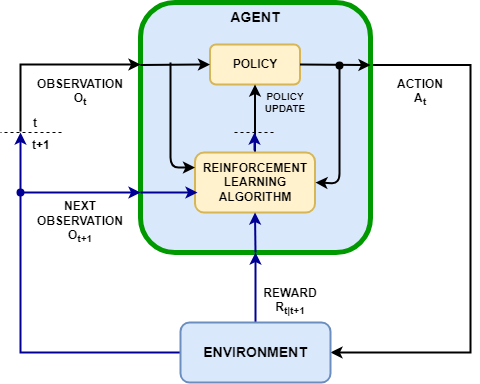
\includegraphics[width=.42\textwidth]{images/rl_scheme.png}
  \caption{RL Agent Scheme}
  {Source: Mathworks\footnotemark} \label{fig:rl_scheme}
\end{figure}
\footnotetext{\url{https://it.mathworks.com/help/reinforcement-learning/ug/create-agents-for-reinforcement-learning.html}}

However, RL has its own set of challenges. The most common one is the
convergence to a local minimum in the reward function. This means that the agent
might learn a suboptimal strategy that is not the best one. Moreover, RL is not explainable,
meaning that we can't understand why the agent took a specific action in a
specific situation.

Another issue with RL is the cost of training. Since the agent learns through trial
and error, it needs to perform a large number of actions to explore the
environment and learn the best strategy. This can be computationally expensive and
time-consuming, especially for complex problems with many variables and states. Moreover,
once the agent is trained, its adaptability to new environments or situations is
limited, as it is optimized for a specific reward function and environment
configuration.

\paragraph{Literature:}
an example of a problem similar to the one presented in this thesis, solved
using Reinforcement Learning, can be found in the paper ``DeliverAI: a
distributed path-sharing network based solution for the last mile food delivery
problem" by Ashman et al. \cite{mehra2024deliveraireinforcementlearningbased}.

They aimed at solving the last-mile delivery problem by developing a distributed
path-sharing network based on Reinforcement Learning. Their approach uses a multi-agent
system to optimize delivery routes and schedules, considering factors such as
traffic congestion, delivery time windows, and vehicle capacity.

However, their model simplifies the real-world scenario by assuming fixed delivery
locations and known traffic patterns, which may not accurately reflect the
dynamic and uncertain nature of real-world logistics environments. Moreover,
their approach requires extensive training and tuning to achieve optimal
performance.

\subsection{Planning in LLM}
\label{sub:planning_in_llm}

LLMs are trained on vast amounts of textual data and have demonstrated remarkable
performance across a wide range of language tasks, from translation and
summarization to reasoning and problem-solving. This success has naturally led researchers
to explore whether these models can be repurposed for more complex, multi-step
decision-making problems that require planning.

The key idea is that the same abilities that allow LLMs to understand and
generate language can be harnessed to decompose a planning task into
intermediate steps, reason about the consequences of actions, and even generate
entire action sequences with minimal or no task-specific training.

\subsubsection{Chain-of-Thought Reasoning}

One of the most influential ideas for using LLMs in planning is chain-of-thought
(CoT) prompting. Instead of asking the model to jump directly from a problem
statement to a final answer, CoT prompting encourages the model to ``think aloud"
by generating intermediate reasoning steps. This decomposition can help in planning
problems where the solution involves multiple, logically connected steps.

This was first discovered by Wei et al. \cite{wei2023chainofthoughtpromptingelicitsreasoning},
who demonstrated that prompting the LLM to 'answer step by step' led to improved
performance on mathematical problems compared to requesting only the final
answer. They also showed that this step-by-step approach could be applied to other
fields, ultimately giving rise to Chain-of-Thought (CoT) reasoning.

\paragraph{``Reasoning" Models}
Reasoning-focused LLMs are trained to generate multiple Chain-of-Thought (CoT) steps,
exploring different solution paths before selecting the most optimal one, often using
Reinforcement Learning (RL) \cite{deepseekai2025deepseekr1incentivizingreasoningcapability}
techniques such as RLHF (Reinforcement Learning from Human Feedback) or self-consistency
methods during the training.

This approach enhances both accuracy and explainability, as the model
articulates its reasoning process while still operating as a generative AI
system. Expanding on this concept, reasoning models can integrate external tools,
memory, and API calls, forming what is commonly referred to as an LLM Agent,
capable of autonomous decision-making and real-world interaction.

Last and more famous reasoning models released to the public are by:
\begin{itemize}
  \item \textbf{OpenAI}: o1\footnote{\url{https://openai.com/o1/}}, o1-mini\footnote{\url{https://openai.com/index/openai-o1-mini-advancing-cost-efficient-reasoning/}}
    and o3-mini\footnote{\url{https://openai.com/index/openai-o3-mini/}} are reasoning
    models designed to enhance logical problem-solving capabilities. o1 is
    tailored to tackle complex problems across various domains, offering robust reasoning
    skills. Building upon this foundation, o3-mini provides a more cost-effective
    and faster alternative;

  \item \textbf{DeepSeek}: DeepSeek-R1\footnote{\url{https://github.com/deepseek-ai/DeepSeek-R1}},
    is a notable AI development from a startup\footnote{\url{https://www.deepseek.com/}}.
    Released in early 2025, DeepSeek-R1 is recognized for its powerful reasoning
    and coding skills, achieved at a fraction of the development cost compared to
    other leading models. Its open-source nature and efficiency have made it a
    significant player in the AI landscape.
\end{itemize}

\subsubsection{Zero-Shot and Few-Shot Planning}
In zero-shot planning, LLMs generate action sequences by utilizing their extensive
pretraining on text and code, effectively inferring plausible step-by-step
solutions to given tasks. Few-shot planning further enhances this by providing LLMs
with a small set of demonstrations, enabling them to generalize patterns and
improve their action sequencing capabilities.

However, while LLMs can produce reasonable plans, their direct applicability to
embodied environments remains challenging. Huang et al.
\cite{huang2022languagemodelszeroshotplanners} highlight the limitations of
naive LLM planning, noting that LLMs struggle with real-world constraints,
action feasibility, and long-horizon dependencies. Their work demonstrates that
these shortcomings can be mitigated by leveraging the world knowledge embedded
within LLMs and applying structured guidance, such as constraints on action generation
and feedback-based refinements.

Similarly, Silver et al. \cite{silver2022pddl} extend this inquiry to classical AI
planning domains by evaluating few-shot prompting of LLMs on problems expressed in
the Planning Domain Definition Language (PDDL). Their findings reveal mixed
results: while LLMs can generate syntactically correct PDDL plans in certain domains,
they often fail due to a lack of explicit access to transition models and
logical constraints inherent to planning problems. Nonetheless, their study also
introduces a hybrid approach where LLMs are used to initialize heuristic-based
search planners, demonstrating that even imperfect LLM-generated plans can improve
the efficiency of traditional AI planning methods.

These findings collectively suggest that while LLMs alone are not yet fully capable
of robust autonomous planning, their ability to extract and apply commonsense
knowledge makes them valuable tools for augmenting structured planning
frameworks. By integrating LLM-generated outputs with classical search-based methods,
researchers have shown improvements in planning efficiency and problem-solving
robustness, highlighting a promising direction for future research at the intersection
of language models and automated planning.

\paragraph{Literature:}
in the paper ``Exploring and Benchmarking Planning Capabilities of Large
Language Models" by Bohnet et al.
\cite{bohnet2024exploringbenchmarkingplanningcapabilities}, the authors systematically
analyze the planning capabilities of LLMs through a novel benchmarking suite that
includes both classical planning tasks (expressed in PDDL) and natural language-based
planning problems. Their work highlights the limitations of LLMs in planning, particularly
their tendency to generate suboptimal or incorrect plans despite their strong language
understanding capabilities. To address these shortcomings, they explore various methods
to improve LLM-based planning (including many-shot in-context learning, fine-tuning
with optimal plans, and the use of chain-of-thought reasoning techniques such as
Monte Carlo Tree Search (MCTS) and Tree-of-Thought (ToT)). The results indicate
that, while LLMs struggle with planning in zero-shot and few-shot settings,
their performance significantly improves when provided with structured
demonstrations and reasoning strategies. Moreover, fine-tuning on high-quality
plan data leads to near-perfect accuracy in some cases, even with relatively small
models. However, challenges remain in out-of-distribution generalization, where
models fail to generalize effectively to novel scenarios without additional
training. Their analysis also identifies key failure modes in LLM planning, such
as constraint violations, failure to reach goal states, and incorrect action
sequences, emphasizing the need for better training data curation and reasoning frameworks.

\paragraph{Literature:}
in ``Generalized Planning in PDDL Domains with Pretrained Large Language Models"
by Silver et al. \cite{silver2023generalizedplanningpddldomains}, the authors investigate
whether LLMs, specifically GPT-4, can serve as generalized planners, not just
solving a single planning task, but synthesizing programs that generate plans for
an entire domain. They introduce a pipeline where GPT-4 is prompted to summarize
the domain, propose a general strategy, and then implement it in Python. Additionally,
they incorporate automated debugging, where GPT-4 iteratively refines its generated
programs based on validation feedback. Their evaluation on seven PDDL domains
demonstrates that GPT-4 can often generate efficient, domain-specific planning programs
that generalize well from only a few training examples. The study also finds
that automated debugging significantly improves performance, while the effectiveness
of Chain-of-Thought (CoT) summarization is domain-dependent. Notably, GPT-4 outperforms
previous generalized planning approaches in some cases, particularly when
leveraging semantic cues from domain descriptions. However, limitations remain, especially
in handling domains requiring deeper structural reasoning or non-trivial search processes.
Their results suggest that LLMs can be powerful tools for generalized planning
when properly guided, but refinements in prompting strategies and failure correction
mechanisms are needed.
